\documentclass{article}
\usepackage{tikz}

\usetikzlibrary{positioning}
\usetikzlibrary{arrows}
\usetikzlibrary{arrows.meta}

\tikzset{%
	>={Latex[width=2mm,length=2mm]},
	% Specifications for style of nodes:
	base/.style = {rectangle, rounded corners, draw=black, minimum width=4cm, minimum height=1cm, text centered, font=\sffamily},
	input/.style = {base, fill=blue!30},
	process/.style = {base, fill=red!30},
	output/.style = {base, fill=green!30},
}



\title{Pipeline}
\date{09/02/2018}
\author{Irdi Balla}

\begin{document}
	\maketitle	
	
	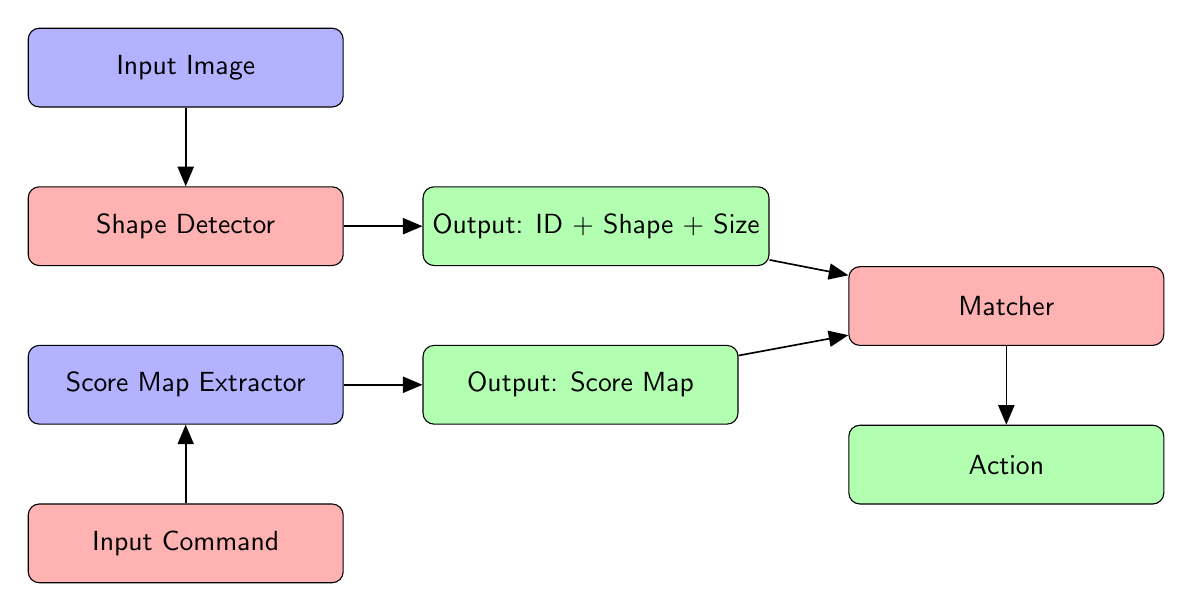
\begin{tikzpicture}[>=triangle 45,font=\sffamily]
		\node (II)[input] {Input Image};
		\node (Shape) [process,below =1cm of II]  {Shape Detector};
		\node (IO) [output,right =1cm of Shape]  {Output: ID + Shape + Size};
		
		\node (ScoreMap) [input,below =1cm of Shape]  {Score Map Extractor};
		\node (IC) [process,below =1cm of ScoreMap]  {Input Command};	
		\node (CO) [output,right =1cm of ScoreMap]  {Output: Score Map};
		
		\node (Matcher) [process, below right=0.0cm and 1cm of IO] {Matcher};
		\node (Action) [output, below = 1cm of Matcher] {Action};
		
		\draw [semithick,->] (II) -- (Shape);
		\draw [semithick,->] (Shape) -- (IO);
		\draw [semithick,->] (IO) -- (Matcher);
		
		\draw [semithick,->] (IC) -- (ScoreMap);
		\draw [semithick,->] (ScoreMap) -- (CO);
		\draw [semithick,->] (CO) -- (Matcher);
		
		\draw [semithick,->] (Matcher) -- (Action);
		
		
	
     \end{tikzpicture}
	
\end{document}
